\chapter{Related Work}
\label{chapter:related-work}

% Amaury: Write an introduction to the chapter

\section{Financial Forecasting}
\label{section:financial-forecasting}

% Amaury: Rewrite

In general, this work involves the use of machine learning to forecast financial
markets. In several efforts, researchers create regression models using
technical or fundamental indicators as training datasets. Examples of regression
techniques are autoregression \cite{burg1968new}, symbolic regression 
\cite{billard2002symbolic}, and linear regression \cite{kutner2004applied}.

The work by Brown, Pelosi and Dirska \cite{brown2013dynamic} uses a Niche
Genetic Algorithm called Dynamic-radius Species-conserving Genetic Algorithm
(DSGA) to select stocks to purchase from the Dow Jones Index. It is important to
mention this work because, in the end, the DSS that is presented in the Proposed
Method does the same kind of recommendation as in their work. More importantly,
Brown, et al., uploaded the dataset that the authors of the present work used to
perform the different experiments. In Section \ref{experiments-and-results} a
comparison to their work is provided, along with many other experiments.

The work by Lu, Lee, and Chiu \cite{Lu2009} point out the complexity of
financial time-series. They note its noisy nature and propose a technique to
reduce this noise based in a two-stage modeling approach using Independent
Component Analysis (ICA) and Support Vector Regression (SVR). Their approach
first uses ICA for generating independent components to identify and remove
those containing the noise, then the remaining components are used to
reconstruct the forecasting variables which now contain less noise and are the
input of the SVR forecasting model. Their work was important for the development
of the Proposed Method, as we believe that the ABM approach can then be used to
diminish the noise in the market, by using a separate class of agents dedicated
to model it.

Lastly, it is imperative to mention the use of Neural Networks in regression
tasks, as it is a technique that has been proved to be very effective for this
kind of problems. O'Connor and Madden \cite{Connor2005} obtained some remarkable
results where they obtained an annual 23.5\% of Rate of Investment on Dow Jones
data used for training and testing. Another example is given by Castillo and
Melin \cite{castillo2001simulation}, where they compare different hybrid
architectures that combine Neural Networks and Fuzzy Logic for the prediction of
financial time-series.

\section{Multi-agent Systems}
\label{section:multi-agent-systems}

% Amaury: Rewrite

The core algorithm of the proposed method is, at its highest level, a
Multi-agent System. It is therefore paramount to mention some works which use
MAS for the forecast or understanding of financial markets.

Klingert and Meyer \cite{Klingert_2012} implement a MAS to analyze the effect of
two market mechanisms: the continuous double auction and logarithmic market
scoring rule. The purpose of the agent-based simulation model is to see the
effect on the number of trades, the accuracy of prediction markets and the
standard deviation of the prices in order to prove three hypothesis that they
propose. In the end, due to a higher amount of trades and lower standard
deviation of the price, their results indicate that the logarithmic market
scoring rule seems to have an advantage over the other mechanism.

Sherstov and Stone \cite{Sherstov2005} present three automated stock-trading
agents which follow different strategies to predict financial markets, and are
compared. The first agent uses Reinforcement Learning, the second a
Trend-following strategy, and the last one Market-making. These agents are part
of a MAS where the better performing agent is chosen for the testing phase. It
is noteworthy to mention that their strategy was used in a live competition and
won.

Kendall and Su \cite{Kendall2003} use a MAS to simulate stock markets within
which stock traders are modeled as heterogeneous adaptive artificial agents. On
average, 80\% of the artificial stock traders were able to trade using
successful trading strategies which brings the investors higher returns compared
to a simple buy-and-hold strategy.

The authors of this work gained useful knowledge about MAS from two theses. The
first one is the work from Grothmann \cite{Grothmann2002}, ``Multi-agent Market
Modeling based on Neural Networks.'' This work served as inspiration for the
architecture of the Proposed Method. The second thesis is Boer-Sorb{\'{a}}n's
``Agent-Based Simulation of Financial Markets,'' which gave an overview of
approaches to describe and understand financial market's dynamics, and motivated
the authors of this work to use the approach of Agent-based Computation to
perform financial forecast.

As a final mention, Samanidou, et. al. \cite{Samanidou_2007}, provides the
reader a very comprehensive overview of Agent-based Modeling, where different
techniques to perform this kind of models are discussed.

\section{Genetic Algorithms}
\label{section:genetic-algorithms}

% Amaury: Rewrite

In the Proposed Method, Genetic Programming is used to generate the Membership
Functions (MF) of the Fuzzy Inference Systems that act as the agents'
functions. The use of Evolutionary Algorithms to generate MF has been proposed
before in several works. What follows is the mention of two works which use
Genetic Algorithms to perform such a task, and in the next Subsection, one can
find more specialized works where Genetic Programming is used.

Thrift \cite{Thrift1991} explores a nowadays widely used technique which
involves the use of a Genetic Algorithm (GA) to discover the parameters of the
Membership Functions (MF) in a Fuzzy Inference System to obtain a better
performance. Homaifar and McCormick \cite{Homaifar1995} go further and use GA to
simultaneously design the MF and the rule sets for fuzzy logic controllers.

\section{Intuitionistic Fuzzy Systems}
\label{section:related-work-intuitionistic-fuzzy-systems}

% Amaury: Rewrite

There are some noteworthy toolkits for the creation of FISs, and this Section
gives a brief description of the ones that have had the strongest influence to
the present work.

Wagner presents a robust implementation of FISs developed in Java in
\cite{Wagner2013}. The authors of the present work have used this particular
toolkit for comparisons in the capabilities of the IFIS to model uncertainty
against type-1 FISs and interval type-2 FISs in
\cite{Hernandez-Aguila2016}. Although the toolkit does not provide many tools
for representing a FIS graphically or for interacting with one, the
implementation provides libraries for building type-1, interval type-2, and
generalized type-2 fuzzy systems.

Moreover, the work by Castro et al. \cite{castro2007interval} provides the same
capabilities as the work by Wagner, but in this case it is an implementation in
Matlab. A direct disadvantage of using this programming language is that Matlab
is not a free nor open source software.  Nevertheless, the language is still
widely used in the scientific community. Furthermore, this implementation
follows an interface similar to the one provided by Matlab's fuzzy logic
toolbox, and provides more robust graphical implementations than the current
version of Wagner's toolkit.

The authors of the present paper have worked in a particular way of achieving
this type of systems, and the method is described in \cite{Hernandez-Aguila2016}
and \cite{Hernandez-Aguila2017-2}.

\subsection{Membership and Non-Membership Functions Design}
\label{subsection:related-work-membership-and-non-membership-functions-design}

The most common approach to graphically representing an IFS is by
lattices. Examples of this type of representation can be found in the works by
I. Despi et al. \cite{Despi2013}, and G. Deschrijver et
al. \cite{Deschrijver2004}. This is a popular approach to graphically represent
an IFS as it enables more compact and concise mathematical expressions. Another
representation that is suitable for mathematical processes is that of a matrix,
and is discussed in detail in the works by R. Parvathi et al. \cite{Parvathi2014},
G. Çuvalcioglu et al. \cite{Yilmaz2015}, and S. Yilmaz et al. \cite{Yilmaz2015a}.

IFSs that are graphically represented like membership functions are usually
represented in Mamdani FISs, and some example works are the ones by
K. T. Atanassov \cite{Atanassov1986}, and H. Davarzani and M. A. Khorheh
\cite{Davarzani2013}. This notation can be suitable for representing an
architecture of an IFIS, but if the plot is in black and white, or in greyscale,
the reader can get confused by the membership and non-membership plots. This
problem can be alleviated by plotting the membership and non-membership
functions in separate plots, as in the works by O. Castillo et
al. \cite{castillo2007intuitionistic}, and M. Akram et al. \cite{Akram2014}.

There are several other graphical representations of IFSs, such as by radar
charts, as in the work by V. Atanassova \cite{Atanassova2010}, and by
geometrical representations, orthogonal projections and three-dimensional
representations, as can be found in the work by E Szmidt and J. Kacprzyk
\cite{Szmidt2000}.

Some applications of IFSs in the area of medical sciences can be found in the
works by E. Szmidt and J. Kacprzyk \cite{Szmidt2001}, C. M. Own \cite{Own2009},
and D. D. Chakarska and L. S. Antonov \cite{Antonov1995}. In the area of group
decision making, we have an example in the work by Z. Xu \cite{Xu2007}. IFSs
have also been used in word recognition, in the area of artificial vision, as in
the example work of L. Baccour et al. \cite{Baccour2008}.

This work proposes that IFSs, in a Mamdani IFIS, should follow an approach
similar to that found in the work by K. T. Atanassov \cite{Atanassov2003}, where
the membership is plotted as is commonly done in a traditional FIS, but the
non-membership function should be plotted as 1-υA. The reason behind this
decision is that the non-membership function should be easily differentiated
from the membership function, while seeing both functions in the same plot. An
implementation of an IFIS that uses this approach for representing IFSs for a
Mamdani IFIS can be found in the work by A. Hernandez-Aguila and
M. Garcia-Valdez \cite{Hernandez-aguila}.

In Figure \ref{figure:traditional-set-as-ifs}, one can see how a traditional
fuzzy set can be constructed using the proposed approach. A Gaussian membership
function with mean of 50 and a standard deviation of 15 is depicted.

\begin{figure}
\caption{A traditional fuzzy set represented as an intuitionistic fuzzy set}
\centering
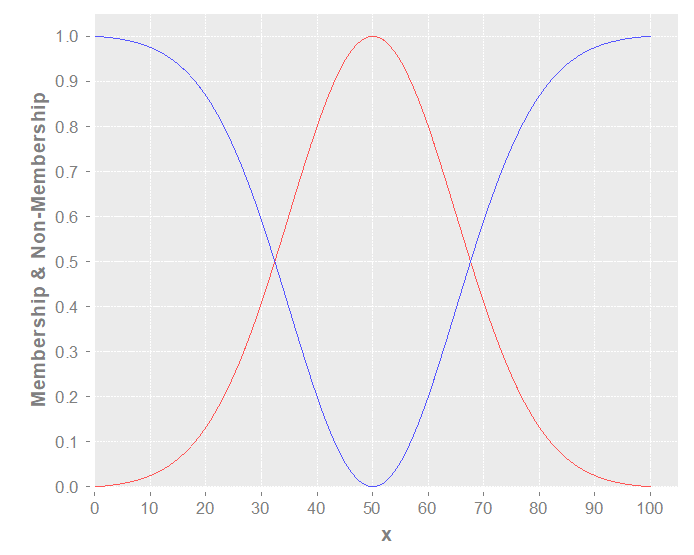
\includegraphics[width=0.7\textwidth]{img/traditional-set-as-ifs.png}
\label{figure:traditional-set-as-ifs}
\end{figure}

Figure \ref{figure:example-of-ifs} is the first case of an IFS that cannot be
considered a tradi-tional fuzzy set. The red line represents the membership
function, while the blue line represents the non-membership function. As can be
seen, the Gaussian membership function does not have a kernel, meaning that its
highest valued member does not equal to 1. In this case, its highest valued
member equals to 0.7, and for the non-membership function, its highest valued
member equals to 0.3. The Gaussian membership function is constructed with a
mean of 50 and a standard deviation of 15. For the non-membership function, it
is con-structed with a mean of 30 and standard deviation of 30.

\begin{figure}
\caption{Representation of an intuitionistic fuzzy set}
\centering
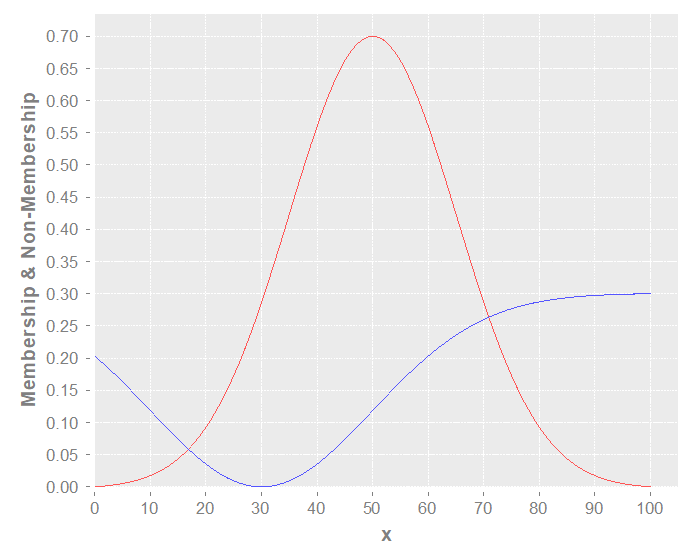
\includegraphics[width=0.7\textwidth]{img/example-of-ifs.png}
\label{figure:example-of-ifs}
\end{figure}
